\ifx\inkludert\undefined
\documentclass[norsk,a4paper,twocolumn,oneside]{memoir}

\usepackage[utf8]{inputenc}
\usepackage{babel}
\usepackage{amsmath,amssymb,amsthm}
\usepackage{mathrsfs}
\usepackage[total={17cm,27cm}]{geometry}
\usepackage[table]{xcolor}
%\usepackage{tabularx}
\usepackage{systeme}
\usepackage{hyperref}
%\usepackage{enumerate}
\usepackage{ifthen}
\usepackage{textgreek}
\usepackage{multirow}
\usepackage{placeins}
\usepackage{caption}

%\usepackage{sectsty}
\setsecheadstyle{\bfseries\large}
%\subsectionfont{\bf\normalsize}

\usepackage{tikz,pgfplots}
\usetikzlibrary{calc}
\usetikzlibrary{arrows.meta}
\def\centerarc[#1](#2)(#3:#4:#5)% Syntax: [draw options] (center) (initial angle:final angle:radius)
    { \draw[#1] ($(#2)+({#5*cos(#3)},{#5*sin(#3)})$) arc (#3:#4:#5); }
\usepackage{pgfornament}

\newcommand{\defterm}[1]{\emph{#1}}

\newcommand{\N}{\mathbb{N}}
\newcommand{\Z}{\mathbb{Z}}
\newcommand{\Q}{\mathbb{Q}}
\newcommand{\R}{\mathbb{R}}
\newcommand{\C}{\mathbb{C}}

\newcommand{\M}{\mathcal{M}} % vektorrom av matriser
\newcommand{\Cf}{\mathcal{C}} % vektorrom av kontinuerlige funksjoner
\renewcommand{\P}{\mathcal{P}} % vektorrom av polynomer
\newcommand{\B}{\mathscr{B}} % basis

\renewcommand{\Im}{\operatorname{Im}}
\renewcommand{\Re}{\operatorname{Re}}

\newcommand{\abs}[1]{|#1|}
\newcommand{\intersect}{\cap}
\newcommand{\union}{\cup}
\newcommand{\fcomp}{\circ}
\newcommand{\iso}{\cong}

\newcommand{\roweq}{\sim}
\DeclareMathOperator{\Sp}{Sp}
\DeclareMathOperator{\Null}{Null}
\DeclareMathOperator{\Col}{Col}
\DeclareMathOperator{\Row}{Row}
\DeclareMathOperator{\rank}{rank}
\DeclareMathOperator{\im}{im}
\DeclareMathOperator{\id}{id}
\DeclareMathOperator{\Hom}{Hom}
\newcommand{\tr}{^\top}
\newcommand{\koord}[2]{[\,{#1}\,]_{#2}} % koordinater mhp basis

\newcommand{\V}[1]{\mathbf{#1}}
\newcommand{\vv}[2]{\begin{bmatrix} #1 \\ #2 \end{bmatrix}}
\newcommand{\vvS}[2]{\left[ \begin{smallmatrix} #1 \\ #2 \end{smallmatrix} \right]}
\newcommand{\vvv}[3]{\begin{bmatrix} #1 \\ #2 \\ #3 \end{bmatrix}}
\newcommand{\vvvv}[4]{\begin{bmatrix} #1 \\ #2 \\ #3 \\ #4 \end{bmatrix}}
\newcommand{\vvvvv}[5]{\begin{bmatrix} #1 \\ #2 \\ #3 \\ #4 \\ #5 \end{bmatrix}}
\newcommand{\vn}[2]{\vvvv{#1_1}{#1_2}{\vdots}{#1_#2}}

\newcommand{\e}{\V{e}}
\renewcommand{\u}{\V{u}}
\renewcommand{\v}{\V{v}}
\newcommand{\w}{\V{w}}
\renewcommand{\a}{\V{a}}
\renewcommand{\b}{\V{b}}
\newcommand{\x}{\V{x}}
\newcommand{\0}{\V{0}}

\newenvironment{amatrix}[1]{% "augmented matrix"
  \left[\begin{array}{*{#1}{c}|c}
}{%
  \end{array}\right]
}

\newcommand{\boks}[1]{\framebox{\strut $#1$}}

% \newcounter{notatnr}
% \newcommand{\notatnr}[2]
% {\setcounter{notatnr}{#1}%
%  \setcounter{page}{#2}%
% }

\newtheorem{thm}{Teorem}[chapter]
\newtheorem{fishythm}[thm]{«Teorem»}
\newtheorem*{thm-nn}{Teorem}
\newtheorem{cor}[thm]{Korollar}
\newtheorem{lem}[thm]{Lemma}
\newtheorem{prop}[thm]{Proposisjon}
\theoremstyle{definition}
\newtheorem{exx}[thm]{Eksempel}
\newtheorem*{defnx}{Definisjon}
\newtheorem*{oppg}{Oppgave}
\newtheorem*{merkx}{Merk}
\newtheorem*{kommentarx}{Kommentar}
\newtheorem*{spmx}{Spørsmål}

\newenvironment{defn}
  {\pushQED{\qed}\renewcommand{\qedsymbol}{$\triangle$}\defnx}
  {\popQED\enddefnx}
\newenvironment{ex}
  {\pushQED{\qed}\renewcommand{\qedsymbol}{$\triangle$}\exx}
  {\popQED\endexx}
\newenvironment{merk}
  {\pushQED{\qed}\renewcommand{\qedsymbol}{$\triangle$}\merkx}
  {\popQED\endmerkx}
\newenvironment{spm}
  {\pushQED{\qed}\renewcommand{\qedsymbol}{$\triangle$}\spmx}
  {\popQED\endspmx}

\setlength{\columnsep}{26pt}

\newcommand{\Tittel}[2]{%
\twocolumn[
\begin{center}
\Large
\begin{tabularx}{\textwidth}{cXr}
\cellcolor{black}\color{white}%
\bf {#1} &
#2
\hfill &
\footnotesize TMA4110 høsten 2018
\\ \hline
\end{tabularx}
\end{center}
]}

\newcommand{\tittel}[1]{\Tittel{\arabic{notatnr}}{#1}}

\newcommand{\linje}{%
\begin{center}
\rule{.8\linewidth}{0.4pt}
\end{center}
}


\newcommand{\kapittelemnenavn}{
\footnotesize
\href{https://wiki.math.ntnu.no/tma4110/2018h/}{TMA4110 høsten 2018}
/
\href{http://creativecommons.org/licenses/by-sa/4.0/}{CC BY-SA}
}
\newcommand{\chapternumber}{}

\makechapterstyle{tma4110}{%
 \renewcommand*{\chapterheadstart}{}
 \renewcommand*{\printchaptername}{}
 \renewcommand*{\chapternamenum}{}
 \renewcommand*{\printchapternum}{\renewcommand{\chapternumber}{\thechapter}}
 \renewcommand*{\afterchapternum}{}
 \renewcommand*{\printchapternonum}{\renewcommand{\chapternumber}{}}
 \renewcommand*{\printchaptertitle}[1]{
\LARGE
\begin{tabularx}{\textwidth}{cXr}
\cellcolor{black}\color{white}%
\textbf{\chapternumber} &
\textbf{##1}
\hfill &
\footnotesize\kapittelemnenavn
\\ \hline
\end{tabularx}%
}
 \renewcommand*{\afterchaptertitle}{\par\nobreak\vskip \afterchapskip}
 % \newcommand{\chapnamefont}{\normalfont\huge\bfseries}
 % \newcommand{\chapnumfont}{\normalfont\huge\bfseries}
 % \newcommand{\chaptitlefont}{\normalfont\Huge\bfseries}
 \setlength{\beforechapskip}{0pt}
 \setlength{\midchapskip}{0pt}
 \setlength{\afterchapskip}{10pt}
}
\chapterstyle{tma4110}
\pagestyle{plain}


\newboolean{vis-oppgaver}
\newboolean{vis-losninger}
\setboolean{vis-oppgaver}{true}
\setboolean{vis-losninger}{false}

\newcounter{oppg-kap} % kapittelnummerering for oppgaver
\newcounter{oppgnr}[oppg-kap]
\newcounter{punktnr}[oppgnr]

\newenvironment{oppgave}%
 {\ifthenelse{\boolean{vis-oppgaver}}%
             {\par\noindent\stepcounter{oppgnr}\textbf{\arabic{oppgnr}.}}%
             {\expandafter\comment}}%
 {\ifthenelse{\boolean{vis-oppgaver}}%
             {\par\bigskip}%
             {\expandafter\endcomment}}

\newenvironment{losning}%
 {\ifthenelse{\boolean{vis-losninger}}%
             {\par\noindent\stepcounter{oppgnr}\textbf{\arabic{oppg-kap}.\arabic{oppgnr}.}}%
             {\expandafter\comment}}%
 {\ifthenelse{\boolean{vis-losninger}}%
             {\par\bigskip}%
             {\expandafter\endcomment}}

\newenvironment{punkt}
 {\par\smallskip\noindent\stepcounter{punktnr}\textbf{\alph{punktnr})} }
 {\par}

\newcommand{\kap}[1]{\setcounter{oppg-kap}{#1}\addtocounter{oppg-kap}{-1}\stepcounter{oppg-kap}}

\newcommand{\oppgaver}[1]{%
  \kap{#1}%
  \ifthenelse{\boolean{vis-oppgaver}}%
             {\linje\section*{Oppgaver}}%
             {}}

\usepackage{xr}
\externaldocument{tma4110-2018h}
\newcommand{\kapittel}[2]{\setcounter{chapter}{#1}\addtocounter{chapter}{-1}\chapter{#2}}
\newcommand{\kapittelslutt}{\enddocument}
\begin{document}
\chapterstyle{tma4110}
\pagestyle{plain}
\fi


\kapittel{14}{Systemer av differensiallikninger}
\label{ch:systemer-av-lineare-differensiallikninger}

I dette kapitlet skal vi bruke det vi har lært om lineær algebra til å løse differensiallikninger. 
Det finnes differensiallikninger for nesten alt, men det er kun de aller enkleste som er mulig å løse. 
Et studium av differensiallikninger begynner gjerne med en klassifisering av forskjellige typer likninger, 
slik at man kan bestemme seg for hvilken klasse av likninger man i det hele tatt ønsker å ta i betraktning. 
I prinsippet består denne klassifiseringen av å skrelle vekk likninger som er for kompliserte til å løses. 



\section*{Vektorfunksjoner}
En \defterm{vektorfunksjon} er en funksjon $\V f: \R \to \C^n$: 
\[
\V f(t)=
\begin{bmatrix}
f_1(t) \\ f_2(t) \\ \vdots \\ f_n(t)
\end{bmatrix}
\]
der alle komponentene er funksjoner fra $\R$ til $\C$.

\begin{ex}
Funksjonen 
\[
\V f(t)=
\begin{bmatrix}
\cos t \\ \sin t 
\end{bmatrix}
\qquad 0\leq t \leq 2\pi
\]
tegner enhetssirkelen i $\R^2$. 
\end{ex}

\begin{ex}
Funksjonen 
\[
\V f(t)=e^{it}=\cos t + i\sin t
\qquad 0\leq t \leq 2\pi
\]
tegner enhetssirkelen i det komplekse planet $\C$. 
\end{ex}

\begin{ex}
Funksjonen 
\[
\V f(t)=
\begin{bmatrix}
\cos t \\ \sin t \\ t 
\end{bmatrix}
\qquad 0\leq t 
\]
tegner en oppadgående spiral i $\R^3$. Den starter i origo, og er uendelig lang. 
\end{ex}


\begin{ex}
Funksjonen 
\[
\V f(t)=
\begin{bmatrix}
2t \\ t  
\end{bmatrix}
=
\begin{bmatrix}
2 \\ 1
\end{bmatrix}t
\qquad t \in \R
\]
tegner en den rette linjen utspent av vektoren
\[
\begin{bmatrix}
2 \\ 1
\end{bmatrix}
\]
 i $\R^2$. 
\end{ex}
\begin{ex}
Funksjonen 
\[
\V f(t)=
\begin{bmatrix}
2 \\ 1  
\end{bmatrix}e^t
\qquad t \in \R
\]
tegner den delen av linjen i forrige eksempel som ligger i første kvadrant i $\R^2$. 
\end{ex}


\begin{defnx}
Vi definerer den deriverte av $\V f$ som 
\[
\V f'(t)=
\begin{bmatrix}
f'_1(t) \\ f'_2(t) \\ \vdots \\ f'_n(t)
\end{bmatrix}.
\]
\end{defnx}

\section*{Systemer av differensiallikninger}

I dette kapitlet skal 
\[
A=
\begin{bmatrix}
a_{11} & a_{12} & \cdots & a_{1n} \\
a_{21} & a_{22} & \cdots & a_{2n} \\
\vdots & \vdots & \ddots & \vdots \\
a_{n1} & a_{m2} & \cdots & a_{nn}
\end{bmatrix}
\]
 alltid være en reell matrise. Det blir mer enn komplisert nok. 
 Et \defterm{førsteordens lineært og homogent system av differensiallikninger med konstante koeffisienter} er et sett med $n$ likninger og $n$ ukjente
\[
\begin{bmatrix}
a_{11} & a_{12} & \cdots & a_{1n} \\
a_{21} & a_{22} & \cdots & a_{2n} \\
\vdots & \vdots & \ddots & \vdots \\
a_{n1} & a_{m2} & \cdots & a_{nn}
\end{bmatrix}
\begin{bmatrix}
y_1(t) \\ y_2(t) \\ \vdots \\ y_n(t)
\end{bmatrix}
=
\begin{bmatrix}
y'_1(t) \\ y'_2(t) \\ \vdots \\ y'_n(t)
\end{bmatrix}
\]
På kortform skriver vi enkelt og greit
\[
A\V y=\V y',
\]
og forkorter den lange tittelen til \textit{system}. 
For å løse dette systemet, skal vi bruke en teknikk som ligner på den du brukte når du løste andreordens differensiallikninger på gymnaset. 
Vi hoster enkelt og greit opp løsninger uten noen som helst forklaring på hvor det kommer fra, og viser etterpå at løsningene er korrekte. 
Vi begynner med den enkleste klassen av løsninger, nemlig de konstante.

\begin{defnx}
En konstant funksjon som løser systemet $A\V y=\V y'$, kalles en \defterm{likevektsløsning}.
\end{defnx}

\begin{thm}
Alle $\V x \in \Null A$ er likevektsløsninger av systemet $A\V y=\V y'$. 
\end{thm}
\begin{proof}
Siden $\V x$ er konstant, er $\V x'=0$, og siden  $\V x \in \Null A$, er $A\V x=0=\V x'$.
\end{proof}


Nå tar vi en mer interessant klasse av løsninger.

\begin{thm}
Vektorfunksjonen
\[
\V y(t)=
\V x e^{\lambda t}
\]
er en løsning av systemet 
\[
A\V y=\V y'
\]
hvis og bare hvis $\lambda$ er en egenverdi, og $\V x$ den korresponderende egenvektor, til matrisen A. 
\end{thm}
\begin{proof}
Vi beregner (husk at $e^{\lambda t}$ er en skalar)
\[
A\V y=A\V x e^{\lambda t}=\lambda \V x e^{\lambda t} = \left(\V x e^{\lambda t}\right)'=\V y'.
\]
Omvendt kan vi se at dersom $\V x e^{\lambda t}$ skal være en løsning av systemet, må 
\[
A\V x e^{\lambda t}=\left(\V x e^{\lambda t}\right)'=\lambda \V x e^{\lambda t}, %\qedhere
\]
og hvis vi deler ut  $e^{\lambda t}\neq 0$ får vi
\[
A\V x = \lambda \V x, %\qedhere
\] 
som sier at $\V x$ er en egenvektor med egenverdi $\lambda$.
\end{proof}


\begin{merkx}
Dersom 0 er en egenverdi, blir den korresponderende egenvektoren en likevektsløsning,
og dette er de samme likevektsløsningene som detter ut av nullrommet til $A$.
\end{merkx}


\begin{ex}
Vi løser systemet 
\[
A\V y=\V y'
\]
der 
\[
A=
\begin{bmatrix}
2 & 1  \\
1 & 2 
\end{bmatrix}.
\]
Egenvektorer er som kjent 
\[
c_1
\begin{bmatrix}
1  \\
1 
\end{bmatrix}
\quad \text{og} \quad
c_2
\begin{bmatrix}
1  \\
-1 
\end{bmatrix}
\]
med egenverdier $3$ og $1$, henholdsvis. Derfor er to løsninger av likningssystemet
\[
\V y_1=
c_1
\begin{bmatrix}
1  \\
1 
\end{bmatrix} e^{3t}
\quad \text{og} \quad
\V y=
c_2
\begin{bmatrix}
1  \\
-1 
\end{bmatrix}e^{t}. \qedhere
\]
\end{ex}


Vi tar med en umiddelbar konsekvens av teoremet over.

\begin{thm}
Det er like mange løsninger på formen $\V x e^{\lambda t}$ av 
\[
A\V y=\V y'
\]
som antall lineært uavhengige egenvektorer til $A$.
\end{thm}



\begin{ex}
Matrisen
\[
A=
\begin{bmatrix}
1 & 2 & 2\\  2 &6 & 2 \\ 2 & 2 & 6
\end{bmatrix}
\]
har egenvektorer 
\[
\begin{bmatrix}
0 \\ -1 \\ 1
\end{bmatrix},
\;
\begin{bmatrix}
1 \\ 2 \\ 2
\end{bmatrix}
\quad \text{og} \quad
\begin{bmatrix}
-4 \\ 1 \\ 1
\end{bmatrix}.
\]
med egenverdier henholdsvis $4$, 9 og $0$. Løsningene av $A\V y=\V y'$ er 
\[
c_1
\begin{bmatrix}
0 \\ -1 \\ 1
\end{bmatrix} e^{4t}, \quad
c_2
\begin{bmatrix}
1 \\ 2 \\ 2
\end{bmatrix}e^{9t}
\quad \text{og} \quad
c_3
\begin{bmatrix}
-4 \\ 1 \\ 1
\end{bmatrix}. \qedhere
\]
\end{ex}

Siden både venstre- og høyresiden av systemet $A\V y=\V y'$ er lineærtransformasjoner som tar inn vektoren $\V y$, 
ser vi at lineærkombinasjoner av løsninger også er løsninger.  Dette kalles \defterm{superposisjonsprinsippet}.
Det er derfor naturlig å sette opp følgende definisjon. Av tekniske grunner som vi ikke skal gå inn på, må vi anta at $A$ er diagonaliserbar.

\begin{defnx}
Anta at $A$ er en diagonaliserbar matrise. Vi definerer systemet $A\V y=\V y'$ sin generelle løsning som 
\[
\V y(t)=c_1\V x_1e^{\lambda_1 t}+c_2\V x_2e^{\lambda_2 t}+...+c_n\V x_ne^{\lambda_n t}
\]
der $\V x_k$ er egenvektorene til $A$, med korresponderende egenverdier $\lambda_k$.
\end{defnx}

\begin{kommentarx}
Det går an å vise at for en reell og diagonaliserbar matrise, har vi fått med oss alle løsninger av systemet $A\V y=\V y'$. Men det er for hardt for oss.
\end{kommentarx}


\begin{ex}
Den generelle løsningen til systemet med matrise
\[
A=
\begin{bmatrix}
1 & 2 & 2\\  2 &6 & 2 \\ 2 & 2 & 6
\end{bmatrix}
\]
er
\[
\V y(t)=
c_1
\begin{bmatrix}
0 \\ -1 \\ 1
\end{bmatrix} e^{4t}
+
c_2
\begin{bmatrix}
1 \\ 2 \\ 2
\end{bmatrix}e^{9t}
+
c_3
\begin{bmatrix}
-4 \\ 1 \\ 1
\end{bmatrix}. \qedhere
\]
\end{ex}

\begin{kommentarx}
Dersom $A$ ikke er diagonaliserbar finnes det andre typer løsninger, 
men de ikke så gode å skrive opp med det teoretiske rammeverket vi har bygget til nå. 
Vi skal senere gi et enkelt eksempel der $A$ ikke er diagonaliserbar, for å gi en smakebit på hvordan det fungerer.
\end{kommentarx}

%\begin{merkx}
%Systemet 
%\[
%A\V y=\V y'+\V b
%\]
%der 
%$\V b \in \Col A$, har likevektsløsninger $\V x$ slik at $A\V x=\V b$. Løsninger av systemet kan da skrives på formen
%\[
%\V y(t)=c_1\V x_1e^{\lambda_1 t}+c_2\V x_2e^{\lambda_2 t}+...+c_n\V x_ne^{\lambda_n t}+\V x.
%\] 
%\end{merkx}

I noen tilfeller er det naturlig å spesifisere et punkt $\R^n$ der løsningskurven skal starte. 

\begin{defnx}
Et \defterm{initialverdiproblem} er et likningssystem
\[
A\V y=\V y'
\]
med initialbetingelse
\[
\V y(t_0)=\V y_0,
\]
der $\V y_0 \in \R^n$. En løsning som tilfredsstiller dette kravet, kalles en \defterm{spesiell løsning}.
\end{defnx}


\begin{ex}
Den spesielle løsningen 
\[
\V y(t)=
\begin{bmatrix}
0 \\ -1 \\ 1
\end{bmatrix} e^{4t}
+
\begin{bmatrix}
1 \\ 2 \\ 2
\end{bmatrix}e^{9t}
+
\begin{bmatrix}
-4 \\ 1 \\ 1
\end{bmatrix}
\]
til systemet i forrige eksempel, starter i punktet 
\[
\begin{bmatrix}
-3 \\ 2 \\ 4
\end{bmatrix}
\]
ved $t=0$. \qedhere
\end{ex}

%\begin{defnx}
%Et initialverdiproblemer \defterm{velformulert} dersom det tilfredsstiller følgende krav:
%\begin{itemize}
%\item Problemet har en løsning
%\item Løsningen er entydig
%\item Løsningens oppførsel avhenger av initialbetingelsene på en kontinuerlig måte
%\end{itemize}
%\end{defnx}

\section*{Forskjellige typer løsninger i planet}

Løsninger av diagonaliserbare $2 \times 2$-systemer kan klassifiseres ganske greit. 
Vi skal også ta med et tilfelle der $A$ ikke er diagonaliserbar, for å gi en smakebit på den generelle teorien. 
Det er gunstig å dele inn i forskjellige tilfeller basert på egenverdiene til $A$, se på hva som skjer når $t \to \infty$, 
og plotte noen løsninger i et \defterm{fasediagram}.

\subsubsection*{Reelle og distinkte egenverdier}
Den generelle løsningen er
\[
\V y(t)=c_1\V x_1e^{\lambda_1 t}+c_2\V x_2e^{\lambda_2 t},
\]
der både $c_1$, $c_2$, $\V x_1$, $\V x_2$, $\lambda_1 \neq \lambda_2$ er relle. Vi illustrerer hva som kan skje med tre eksempler.

\begin{ex}
\label{eks_1}
La 
\[
A=
\begin{bmatrix}
2 & 1  \\
1 & 2 
\end{bmatrix}
\]
slik at 
\[
\V y=
c_1
\begin{bmatrix}
1  \\
1 
\end{bmatrix} e^{3t}
+
c_2
\begin{bmatrix}
1  \\
-1 
\end{bmatrix}e^{t}. 
\]
Merk at uansett hvilke kombinasjoner av $c_1$ og $c_2$ vi har, så lenge ikke begge er 0, 
vil alle løsninger reise mot uendelig når $t\to \infty$, altså vekk fra den eneste likevektsløsningen $\V y=0$. 
Vi sier derfor at $\V y$ er en \defterm{ustabil likevektsløsning}. 
Nedenfor er plot av løsningskurver for et par tusen tilfeldige verdier av $c_1$ og $c_2$. 
\end{ex}

\begin{figure}[htbp]
  \begin{center}
	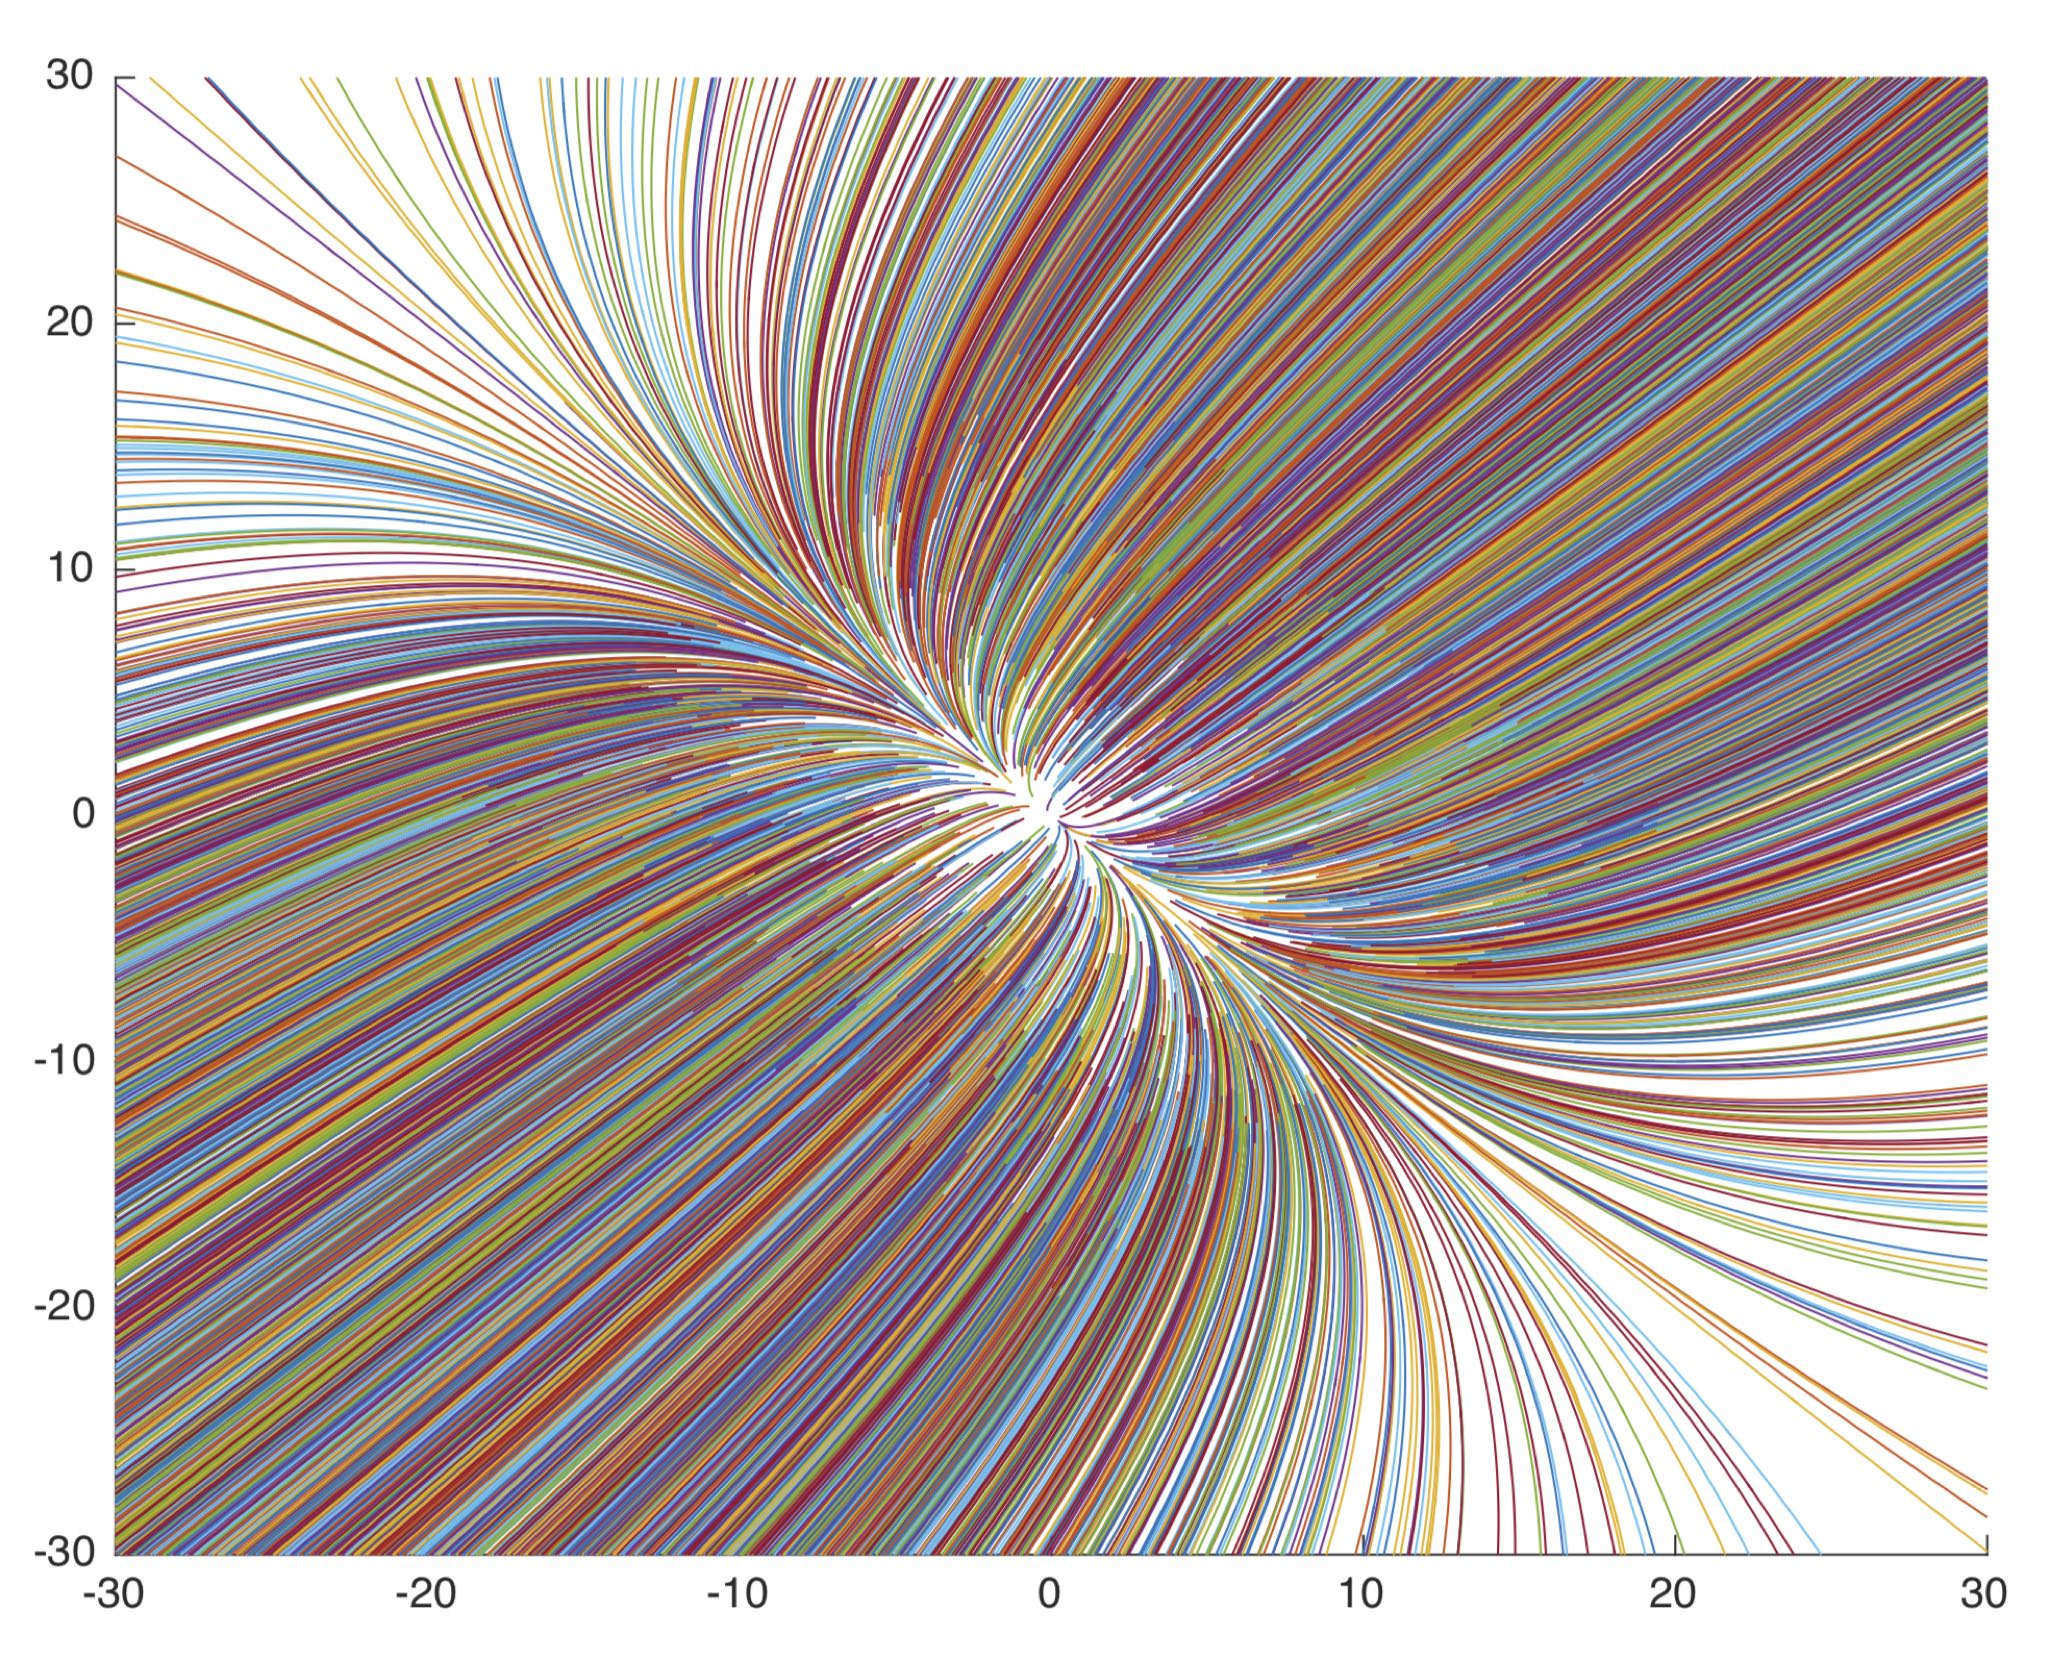
\includegraphics[scale=.1]{eks_1.jpg}
	\captionsetup{labelformat=empty}
	\caption{Eksempel \ref{eks_1}}
	\end{center}
\end{figure}


\begin{ex}
La 
\[
A=
-
\begin{bmatrix}
2 & 1  \\
1 & 2 
\end{bmatrix}
\]
slik at 
\[
\V y=
c_1
\begin{bmatrix}
1  \\
1 
\end{bmatrix} e^{-3t}
+
c_2
\begin{bmatrix}
1  \\
-1 
\end{bmatrix}e^{-t}. 
\]
Merk at uansett hvilke kombinasjoner av $c_1$ og $c_2$ vi har, så lenge ikke begge er 0, 
vil alle løsninger søke mot origo når $t\to \infty$, altså inn mot likevektsløsningen $\V y=0$. 
Vi sier derfor at $\V y$ er en \defterm{stabil likevektsløsning}.
\end{ex}

\begin{ex}
\label{eks_2}
La 
\[
A=
\begin{bmatrix}
1 & -2   \\
-2 & 1
\end{bmatrix}
\]
slik at 
\[
\V y=
c_1
\begin{bmatrix}
1  \\
1 
\end{bmatrix} e^{3t}
+
c_2
\begin{bmatrix}
1  \\
-1 
\end{bmatrix}e^{-t}. 
\]
Merk at så lenge $c_1 \neq 0$, 
vil alle løsninger gå mot uendelig når $t\to \infty$, altså inn mot likevektsløsningen $\V y=0$. 
Men dersom $c_1=0$ og $c_2\neq0$, vil løsningen søke mot origo. Likevektsløsningen $\V y=0$ kalles derfor en
\defterm{ustabil sadel}.
\end{ex}


\begin{figure}[htbp]
  \begin{center}
	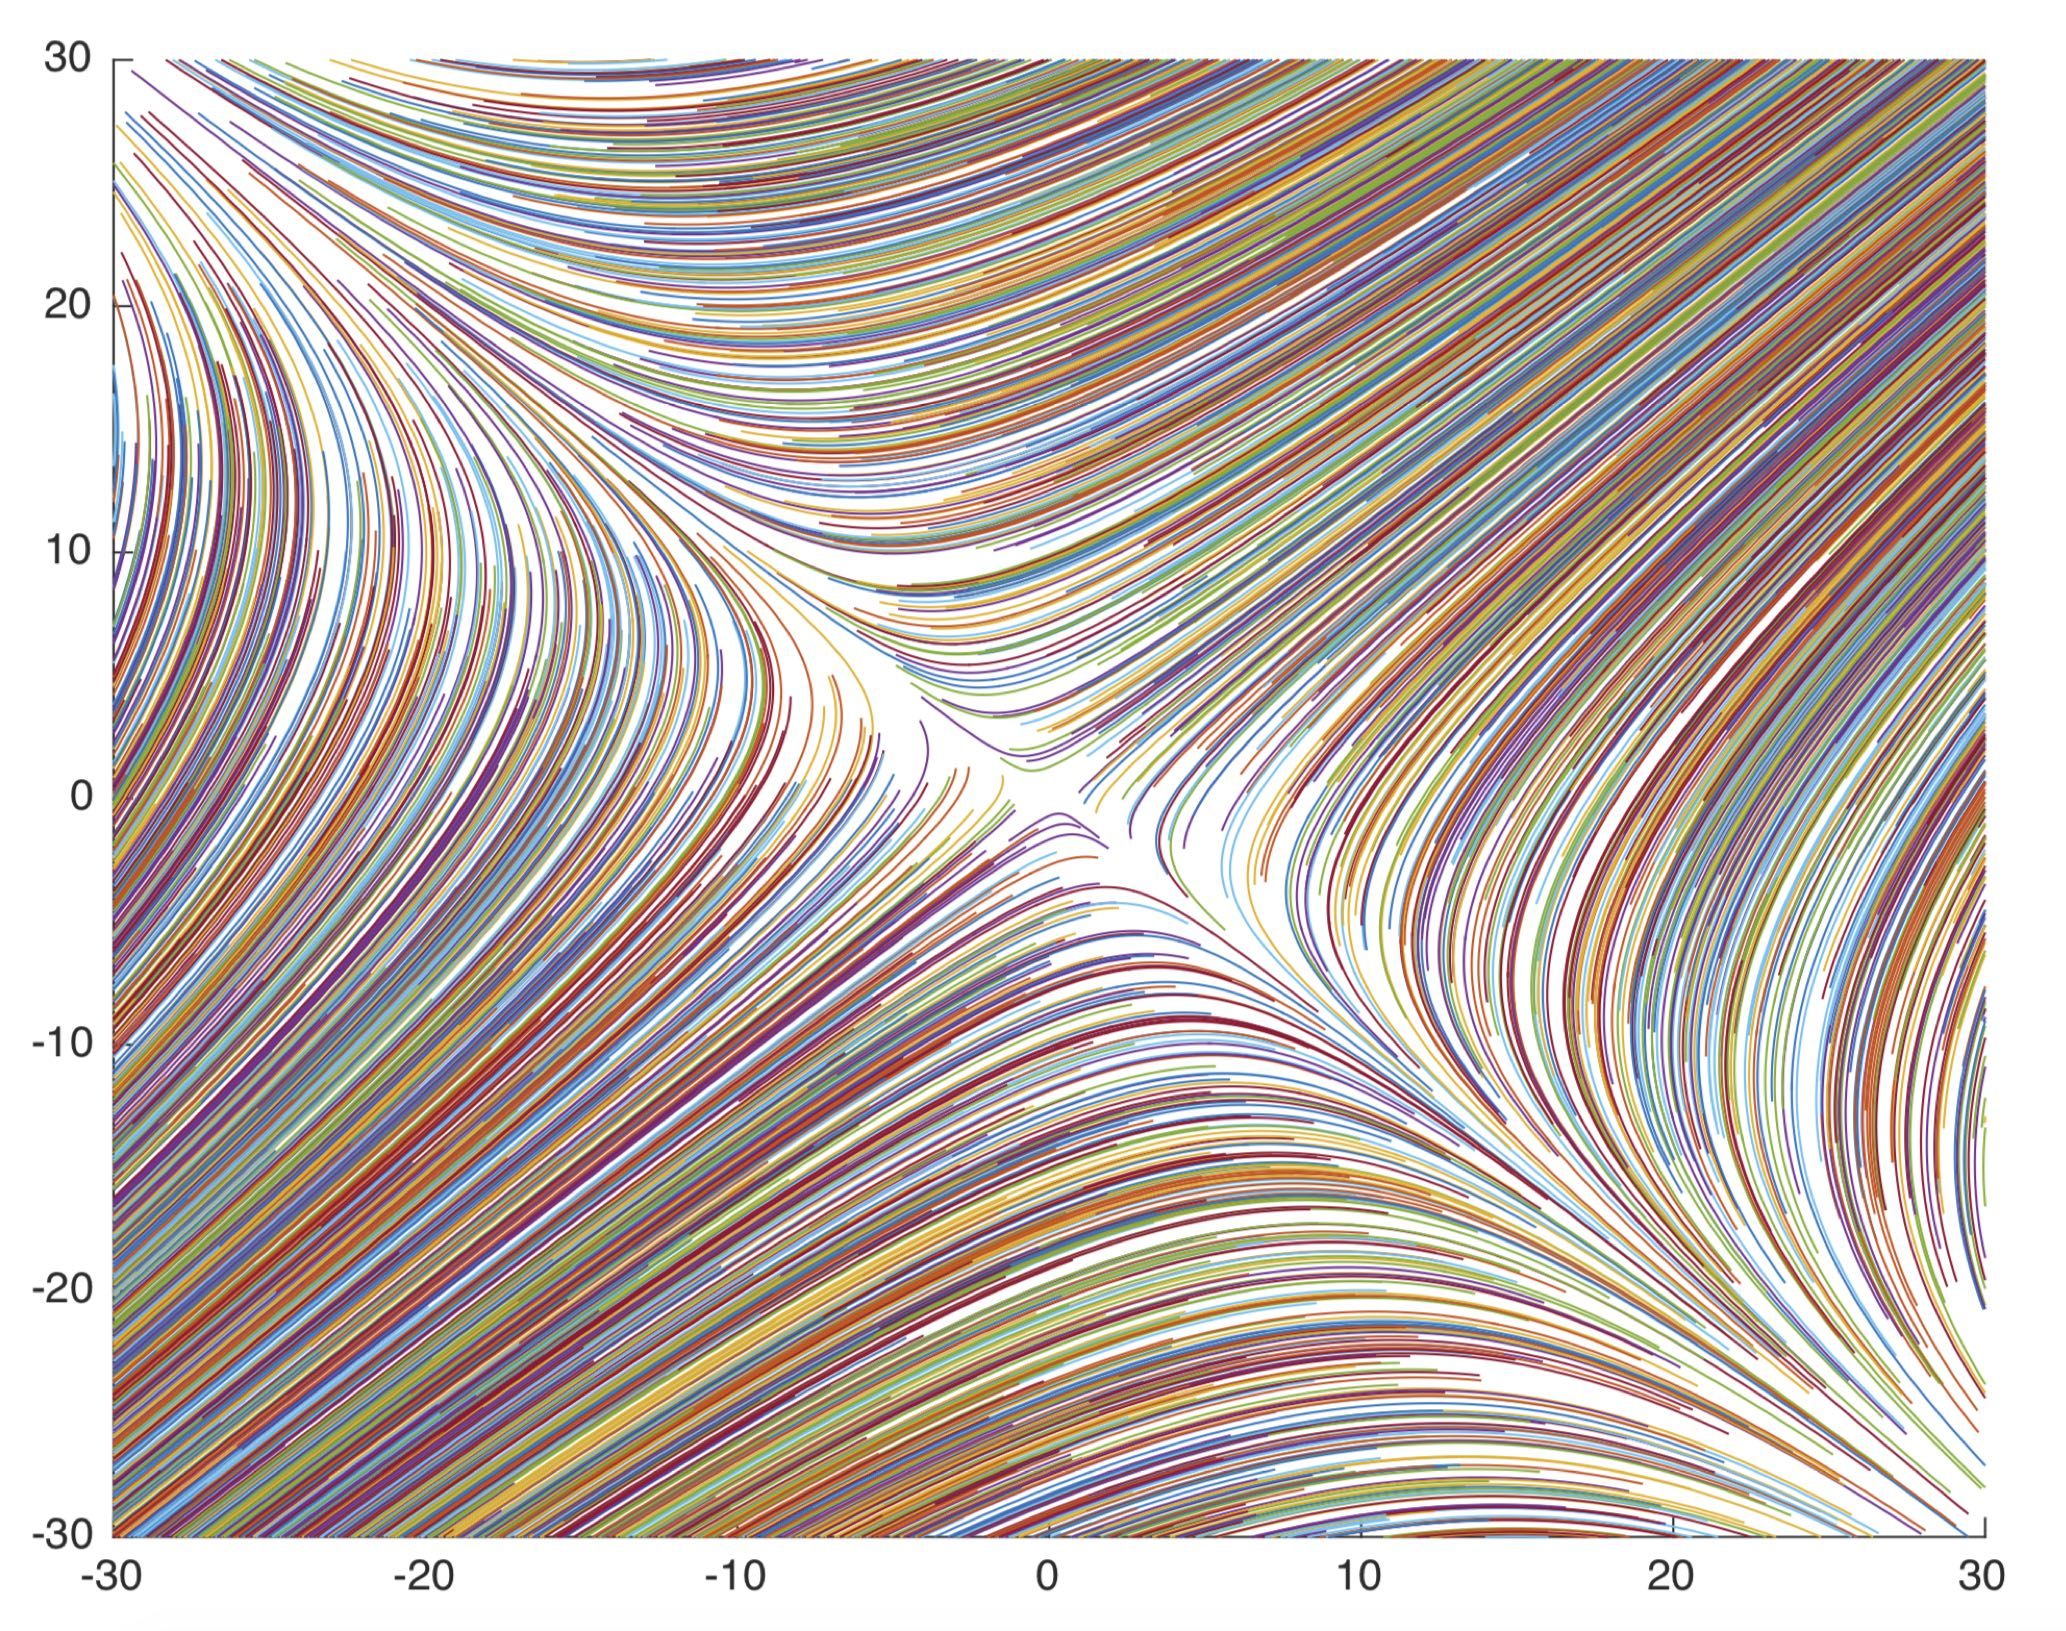
\includegraphics[scale=.1]{eks_2.jpg}	
	\captionsetup{labelformat=empty}
	\caption{Eksempel \ref{eks_2}}
	\end{center}
\end{figure}



\begin{ex}
\label{eks_hm}
La 
\[
A=-\frac{1}{2}
\begin{bmatrix}
3 & 3   \\
3 & 3
\end{bmatrix}
\]
slik at 
\[
\V y=
c_1
\begin{bmatrix}
1  \\
1 
\end{bmatrix} e^{-3t}
+
c_2
\begin{bmatrix}
1  \\
-1 
\end{bmatrix}. 
\]
Merk at så lenge $c_1 \neq 0$, 
vil alle løsninger søke mot likevektsløsningen
\[
\V y=
c_2
\begin{bmatrix}
1  \\
-1 
\end{bmatrix}. 
\]
og ingen mot $\V y=0$ når $t\to \infty$.
\end{ex}

\begin{figure}[htbp]
  \begin{center}
	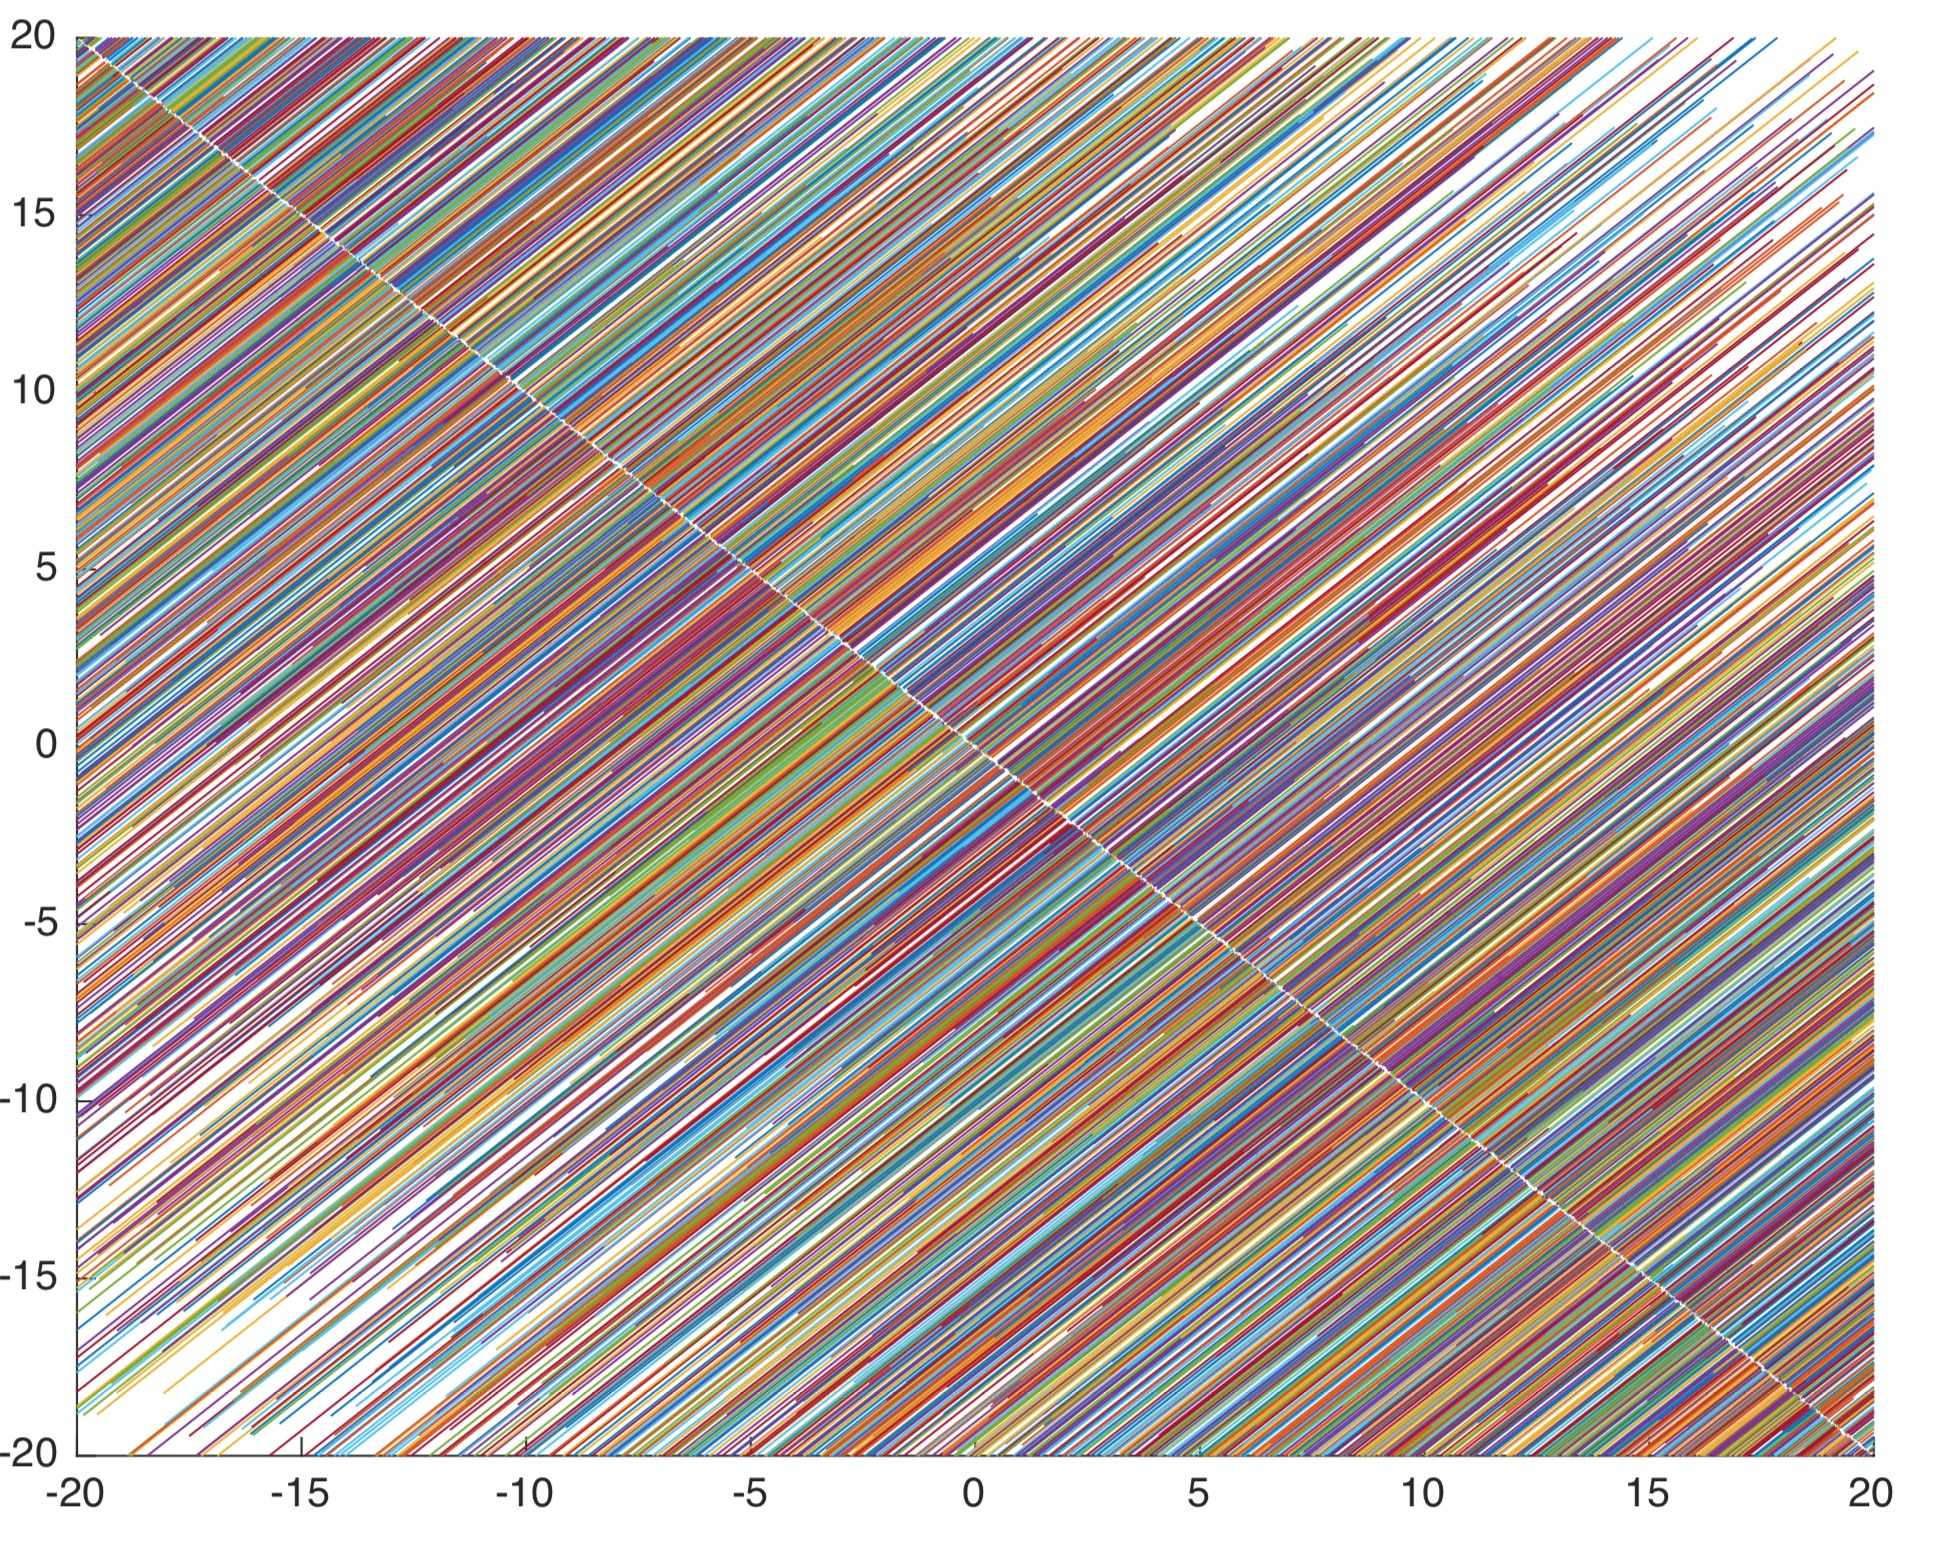
\includegraphics[scale=.1]{eks_hm.jpg}	
	\captionsetup{labelformat=empty}
	\caption{Eksempel \ref{eks_hm}}
	\end{center}
\end{figure}


\subsubsection*{Komplekse egenverdier}
Vi har i øvingsopplegget vist at dersom en reell matrise har komplekse egenverdier, opptrer disse i komplekskonjugerte par.
Du har kanskje lagt merke til at dette også gjelder for de respektive egenvektorene:
\[
A\V x=\lambda \V x \quad \Longleftrightarrow \quad A \overline {\V x} =\overline{ \lambda} \overline {\V  x}
\]

Dette skal vi benytte oss av for å plukke ut relle løsninger. La $\lambda=\alpha+\beta i$ ha egenvektor 
\[\V x=\begin{bmatrix}  x_{1} \\ x_{2}\end{bmatrix}=\begin{bmatrix}  a_{1} \\ a_{2}\end{bmatrix}+i\begin{bmatrix}  b_{1} \\ b_{2}\end{bmatrix},\]
og husk at $e^{\alpha+\beta i}=e^{\alpha}(\cos \beta +i\sin{\beta})$, slik at
\begin{align*}
\V y(t)=\;&c_2\V y_1 +c_2\V y_2 \\ =\;&c_1e^{\lambda t}\V x +c_2e^{\overline{\lambda} t}\overline{\V x} \\ =\;&c_1e^{\alpha t}\left(\begin{bmatrix}  a_{1} \\ a_{2}\end{bmatrix}+i\begin{bmatrix}  b_{1} \\ b_{2}\end{bmatrix}\right)(\cos{\beta t}+i\sin{\beta t})\\+&c_2e^{\alpha t}\left(\begin{bmatrix}  a_{1} \\ a_{2}\end{bmatrix}-i\begin{bmatrix}  b_{1} \\ b_{2}\end{bmatrix}\right) (\cos{\beta t}-i\sin{\beta t}).
\end{align*}
Denne løsningen er pen på papiret, men vi ønsker å kunne visualisere litt, og da hadde det vært praktisk å finne en løsning som var reell istedet. 

Siden  $e^{\lambda t}\V x$ og $e^{\overline \lambda t}\overline{\V x}$ er lineært uavhengige for alle $t$, utgjør de en basis for $\C^2$. La oss søke en reell basis istedet.
Vi kaller den nye basisen $\V v_1$ og $\V v_2$. Velg først $c_1=c_2=\frac{1}{2}$, og sett
\[
\V v_1=e^{\alpha t} \left(\cos \beta t\begin{bmatrix}  a_{1} \\ a_{2}\end{bmatrix}-\sin \beta t\begin{bmatrix}  b_{1} \\ b_{2}\end{bmatrix}\right).
\]
Så velger vi $c_1=-c_2=\frac{1}{2i}$, og setter
\[
\V v_2=e^{\alpha t} \left(\cos \beta t\begin{bmatrix}  b_{1} \\ b_{2}\end{bmatrix}+\sin \beta t\begin{bmatrix}  a_{1} \\ a_{2}\end{bmatrix}\right).
\]
Nå kan vi skrive 
\begin{align*}
\V y(t)=\;&d_1\V v_1 +d_2\V v_2\\ =\;&d_1 e^{\alpha t} \left(\cos \beta t\begin{bmatrix}  a_{1} \\ a_{2}\end{bmatrix}-\sin \beta t\begin{bmatrix}  b_{1} \\ b_{2}\end{bmatrix}\right) 
\\+\;&d_2e^{\alpha t} \left(\cos \beta t\begin{bmatrix}  b_{1} \\ b_{2}\end{bmatrix}+\sin \beta t\begin{bmatrix}  a_{1} \\ a_{2}\end{bmatrix}\right). 
\end{align*}
Merk at siden $\V y_1$ og $\V y_2$ er lineært uavhengige, og forholdet mellom disse og $\V v_1$ og $\V v_2$ er gitt ved
\[
\begin{bmatrix} \V y_2  & \V y_2 \end{bmatrix}\begin{bmatrix} 1 & -i \\ 1 &i \end{bmatrix}=2\begin{bmatrix} \V v_2  & \V v_2 \end{bmatrix},
\]
er også $\V v_1$ og $\V v_2$ lineært uavhengige for alle $t$. Fordelen med den nye basisen er at vi nå enkelt kan skille ut alle reelle løsninger ved å holde oss til relle $d_1$ og $d_2$.


\begin{ex}
\label{eks_3}
La 
\[
A=
\begin{bmatrix}
0 & -1   \\
1 & 0
\end{bmatrix}
\]
som har egenverdier $\pm i$ og egenvektorer 
\[
\begin{bmatrix}
1  \\
i 
\end{bmatrix}
\quad \text{og} \quad
\begin{bmatrix}
1  \\
-i 
\end{bmatrix}. 
\]
Den generelle løsningen til systemet blir 
\begin{align*}
\V y(t)=\;&d_1 \left(\cos t\begin{bmatrix}  1 \\ 0\end{bmatrix}-\sin t\begin{bmatrix} 0 \\ 1\end{bmatrix}\right) 
\\+\;&d_2 \left(\cos t\begin{bmatrix} 0 \\ 1\end{bmatrix}+\sin t\begin{bmatrix}  1 \\ 0\end{bmatrix}\right)\\=\;&d_1\begin{bmatrix} \cos t \\ -\sin t\end{bmatrix}+d_2\begin{bmatrix}  \sin t \\ \cos t\end{bmatrix}=\begin{bmatrix} \cos t & \sin t\\ -\sin t & \cos t\end{bmatrix}\begin{bmatrix} d_1 \\ d_2 \end{bmatrix}.
\end{align*}
Vi ser at denne løsningen starter i punktet $\begin{bmatrix} d_1 \\ d_2 \end{bmatrix}$ ved $t=0$, og kjører deretter i en pen sirkulær bane om origo. 
Merk at kurven er traversert med klokken.
\end{ex}

\begin{figure}[htbp]
  \begin{center}
	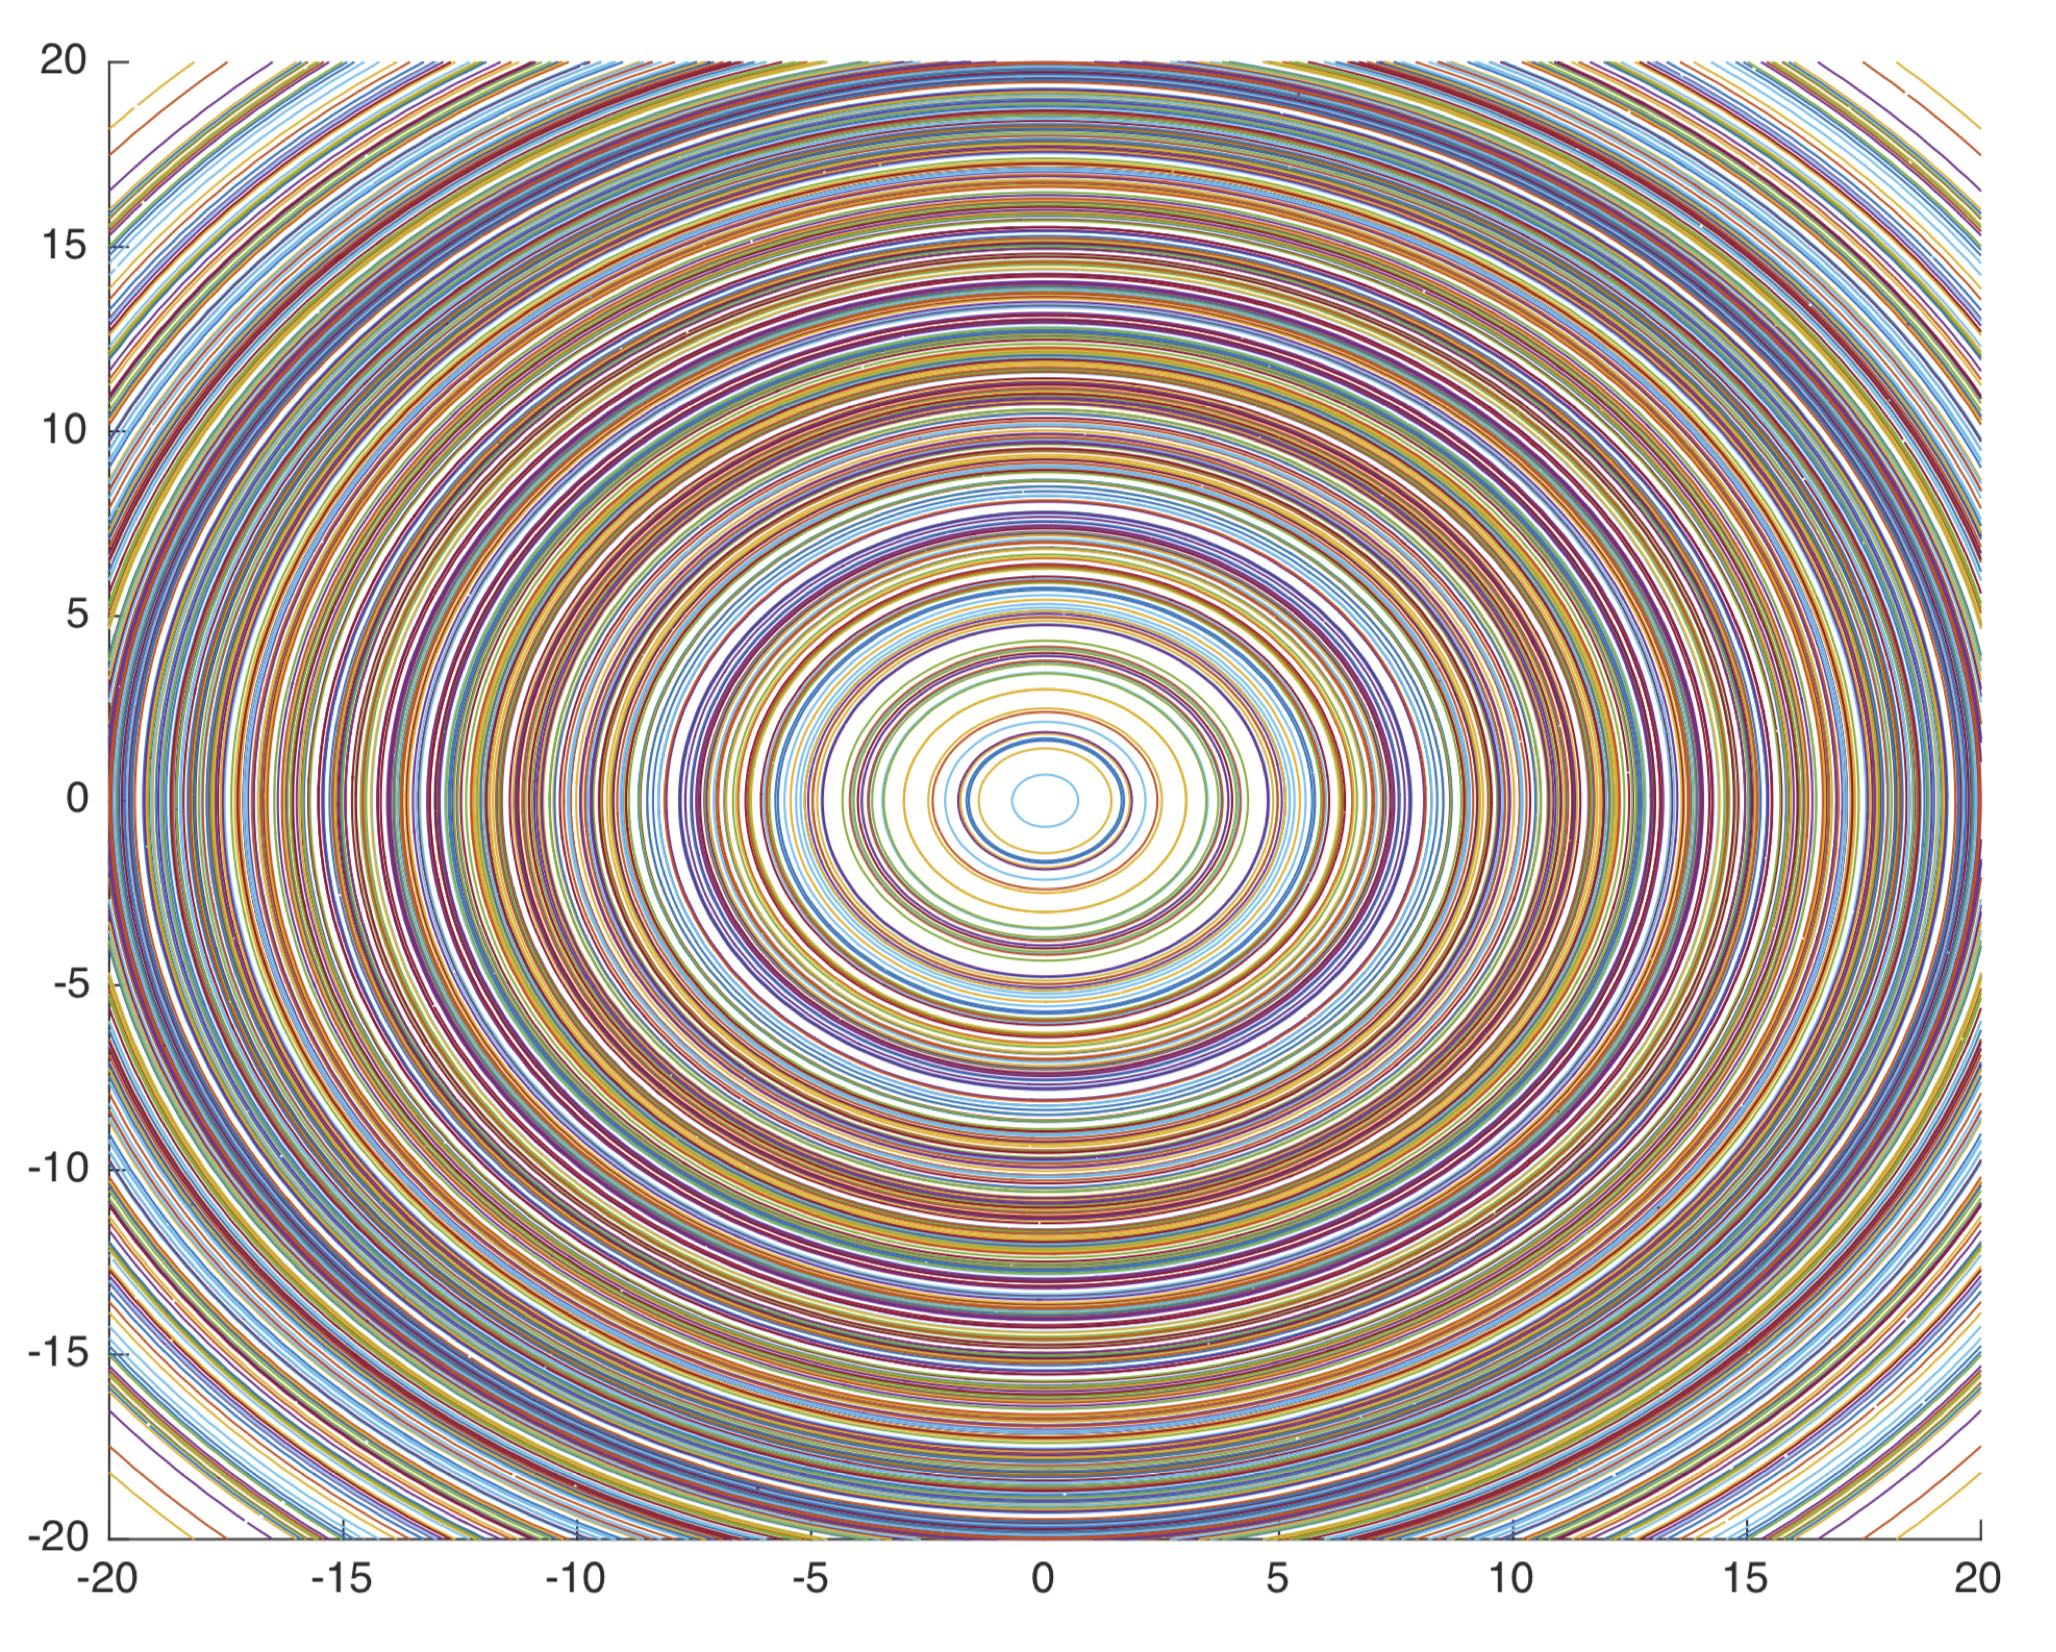
\includegraphics[scale=.1]{eks_3.jpg}
	\captionsetup{labelformat=empty}
	\caption{Eksempel \ref{eks_3}}
	\end{center}
\end{figure}



\begin{ex}
\label{eks_4}
La 
\[
A=
\begin{bmatrix}
1 & -1   \\
1 & 1
\end{bmatrix}
\]
som har egenverdier $1\pm i$ og de samme egenvektorene
\[
\begin{bmatrix}
1  \\
i 
\end{bmatrix}
\quad \text{og} \quad
\begin{bmatrix}
1  \\
-i 
\end{bmatrix}. 
\]
På samme vis som i forrige eksempel blir den generelle løsningen 
\begin{align*}
\V y(t)=\;&d_1e^t\begin{bmatrix} \cos t \\ -\sin t\end{bmatrix}+d_2e^t\begin{bmatrix}  \sin t \\ \cos t\end{bmatrix}\\&=\;e^t\begin{bmatrix} \cos t & \sin t\\ -\sin t & \cos t\end{bmatrix}\begin{bmatrix} d_1 \\ d_2 \end{bmatrix}.
\end{align*}
Denne løsningen starter i punktet $\begin{bmatrix} d_1 \\ d_2 \end{bmatrix}$ ved $t=0$, og kjører deretter i en særdeles vakker sirkulær og utadgående spiral.
\end{ex}


\begin{figure}[htbp]
  \begin{center}
	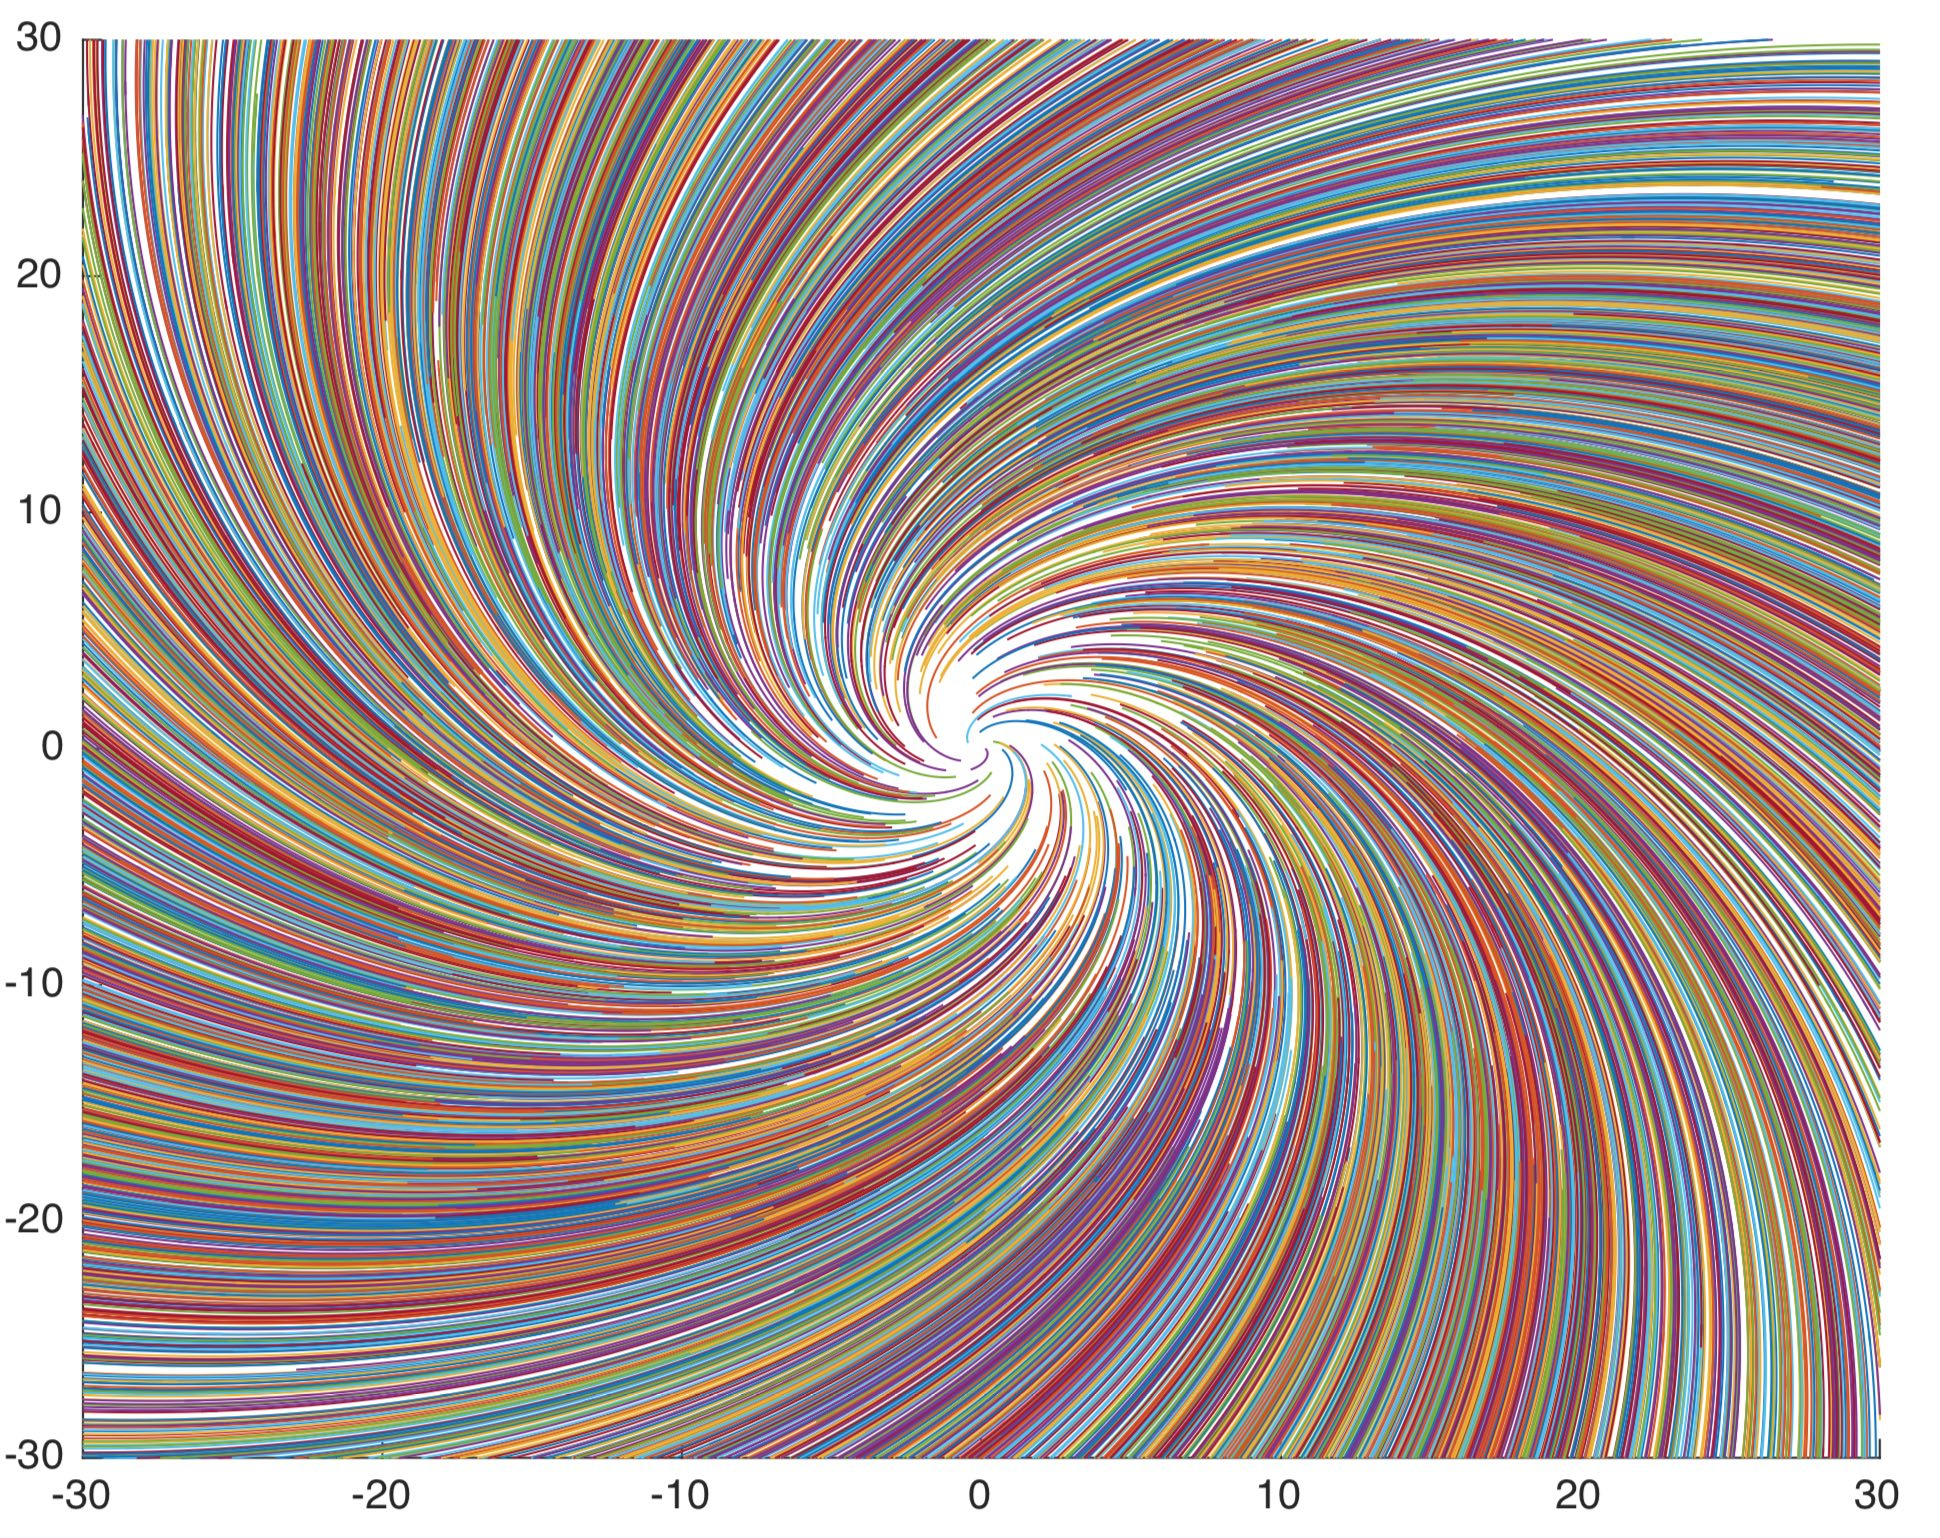
\includegraphics[scale=.1]{eks_4.jpg}
	\captionsetup{labelformat=empty}
	\caption{Eksempel \ref{eks_4}}
	\end{center}
\end{figure}



\begin{ex}
\label{eks_5}
La 
\[
A=
\begin{bmatrix}
-1 & -1   \\
1 & -1
\end{bmatrix}
\]
som har egenverdier $-1\pm i$ og de samme egenvektorene
\[
\begin{bmatrix}
1  \\
i 
\end{bmatrix}
\quad \text{og} \quad
\begin{bmatrix}
1  \\
-i 
\end{bmatrix}. 
\]
På samme vis som i de to forrige eksemplene blir den generelle løsningen 
\begin{align*}
\V y(t)=\;&d_1e^{-t}\begin{bmatrix} \cos t \\ -\sin t\end{bmatrix}+d_2e^{-t}\begin{bmatrix}  \sin t \\ \cos t\end{bmatrix}\\&=\;e^{-t}\begin{bmatrix} \cos t & \sin t\\ -\sin t & \cos t\end{bmatrix}\begin{bmatrix} d_1 \\ d_2 \end{bmatrix}.
\end{align*}
Denne løsningen starter i punktet $\begin{bmatrix} d_1 \\ d_2 \end{bmatrix}$ ved $t=0$, og kjører deretter i en innadgående sirkulær spiral.
\end{ex}


\begin{figure}[htbp]
  \begin{center}
	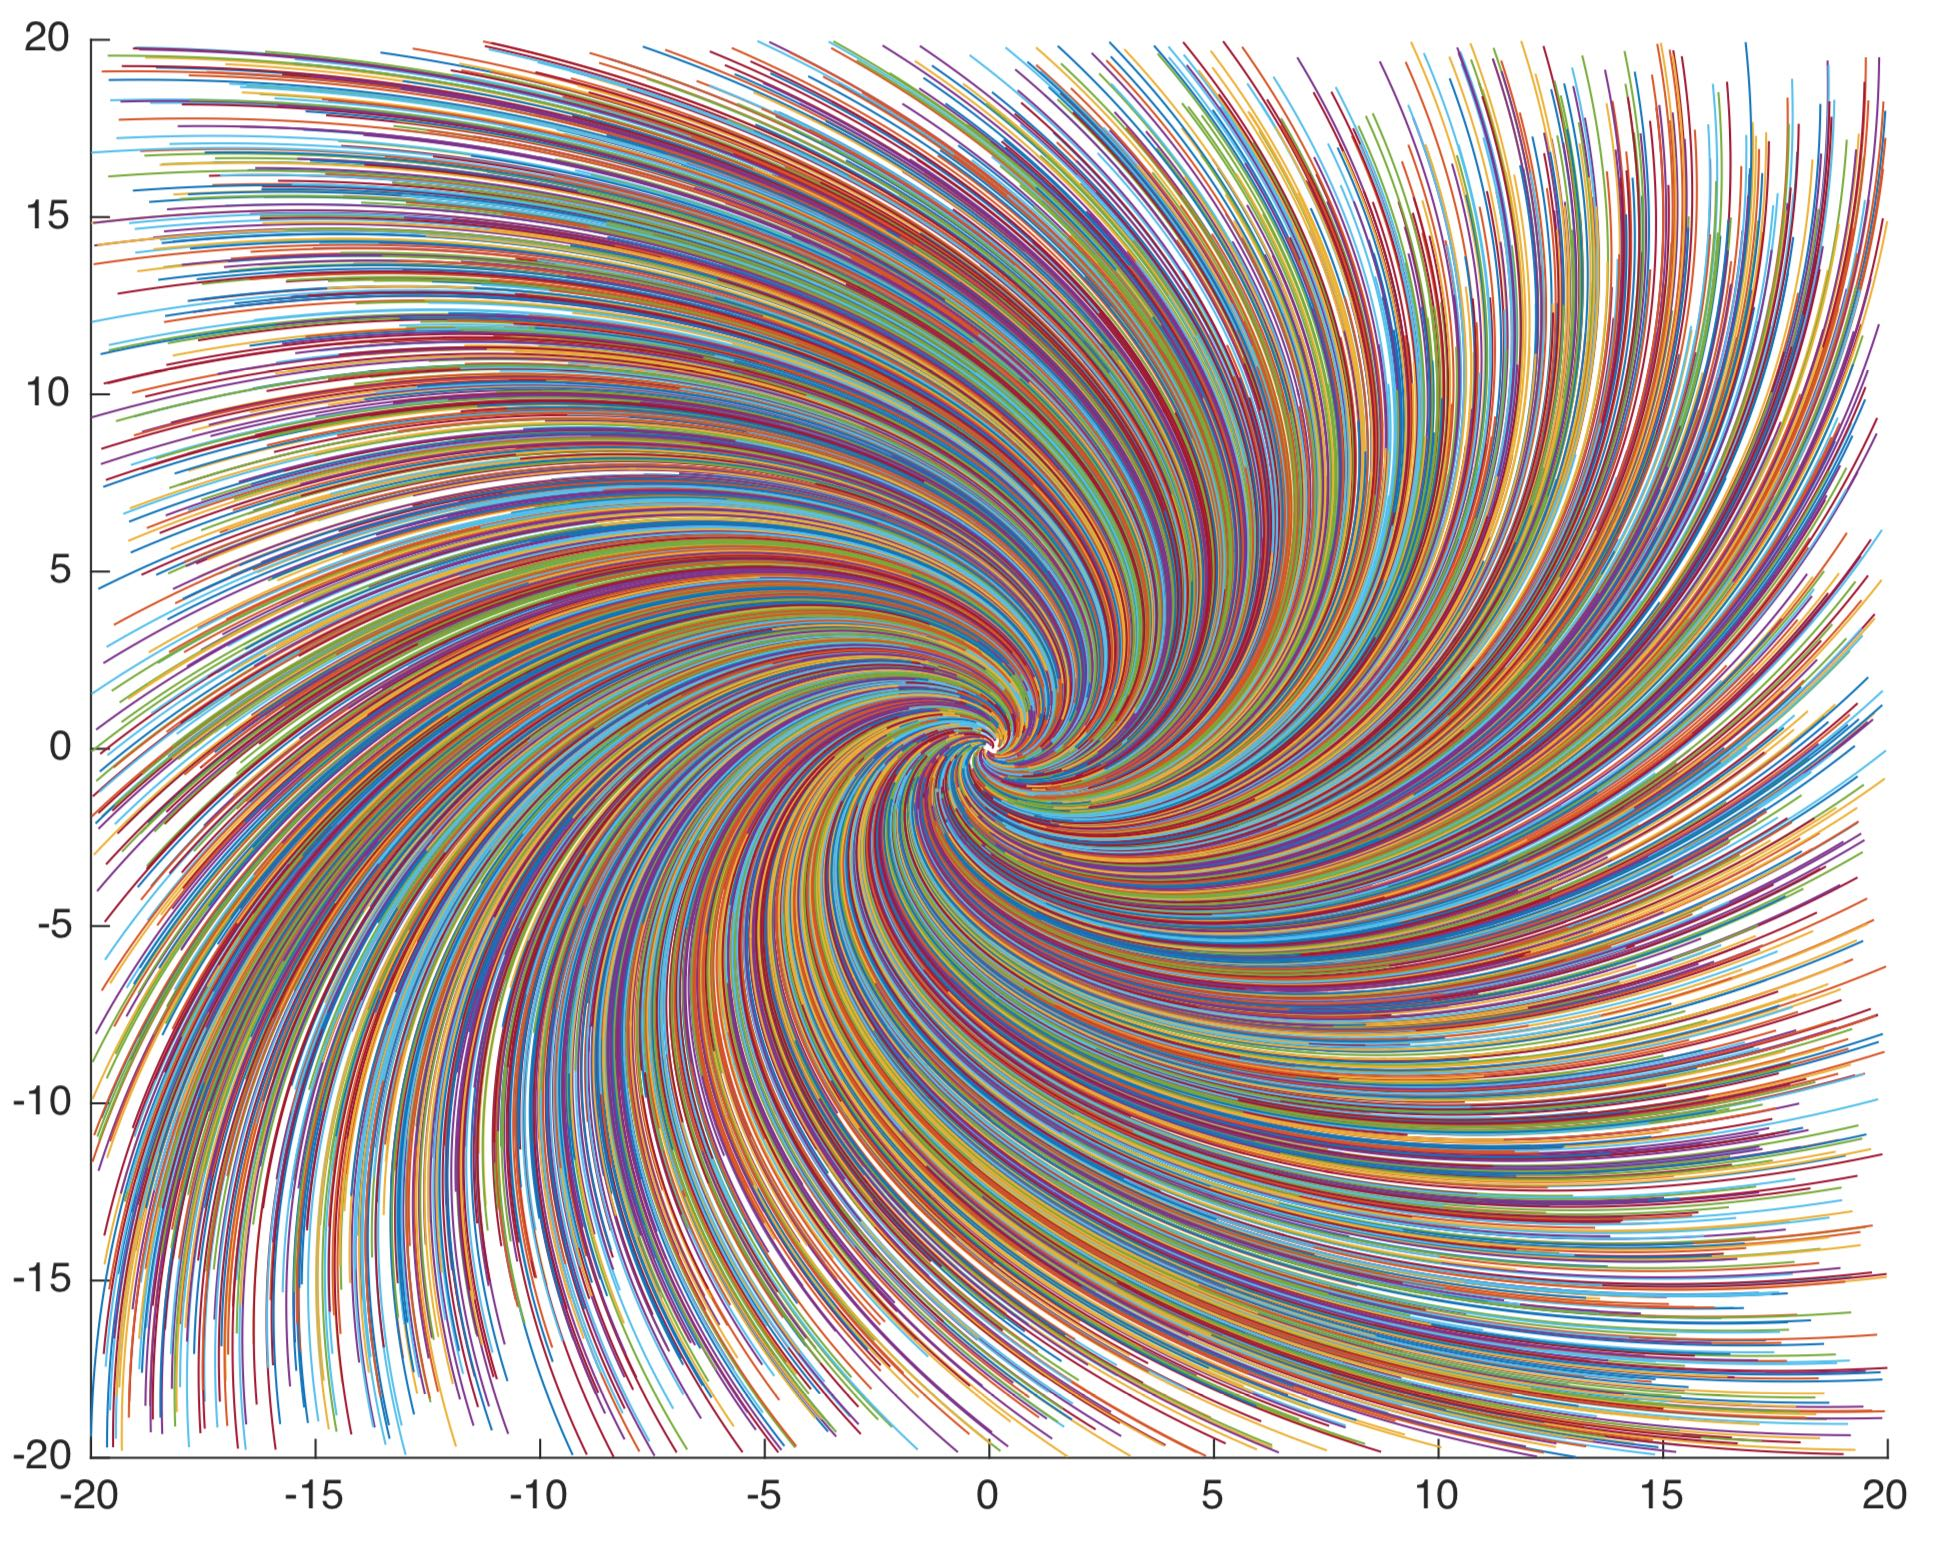
\includegraphics[scale=.1]{eks_5.jpg}
	\captionsetup{labelformat=empty}
	\caption{Eksempel \ref{eks_5}}
	\end{center}
\end{figure}
\subsubsection*{Dobbel egenverdi - for spesielt interesserte!}
Dette tilfellet kan vi egentlig ikke analysere med teorien vi har lært til nå, så du skal slippe å kunne det til eksamen. 
Men vi klarer ikke motstå fristelsen til å  bruke $2 \times 2$-matriser til å ta en smakebit på hva som skjuler seg utenfor pensum. 

\begin{ex}
La 
\[
A=
\begin{bmatrix}
0 & 1   \\
-1 & 2
\end{bmatrix}
\]
som har dobbel egenverdi $1$, men bare en egenvektor
$
\begin{bmatrix}
1  \\
1 
\end{bmatrix}
$.
Hva gjør vi nå?
\end{ex}

For å løse knipen fra forrige eksempel, må vi gjøre noe artig, nemlig introdusere \defterm{generalisert egenvektor}. 
Egenvektoren til $\lambda$ finner man ved å finne nullrommet til $A-\lambda I$. 
For en $2 \times 2$-matrise med defekt egenverdi, er en generalisert egenvektor en vektor i nullrommet til $(A-\lambda I)^2$.
%men ikke i nullrommet til $A-\lambda I$. 

\begin{ex}
La $A$ være som i forrige eksempel. Nullrommet til 
\[
(A-I)^2=
\left(\begin{bmatrix}
-1 & 1   \\
-1 & 1
\end{bmatrix}\right)^2=
\left(\begin{bmatrix}
0 & 0   \\
0 & 0
\end{bmatrix}\right)
\]
er alle vektorer i $\C^2$. Altså er alle vektorer i $\C^2$ 
generaliserte egenvektorer til matrisen $A$.
Vi velger oss en tilfeldig vektor som ikke er parallell med
$
\begin{bmatrix}
1  \\
1 
\end{bmatrix},
$
for eksempel
$
\begin{bmatrix}
-1  \\
1 
\end{bmatrix}.
$
Hvis vi ganger denne inn i $A-I$, får vi 
\[
\begin{bmatrix}
-1 & 1   \\
-1 & 1
\end{bmatrix}
\begin{bmatrix}
-1    \\
 1
\end{bmatrix}
=
\begin{bmatrix}
2    \\
2
\end{bmatrix},
\]
som er en egenvektor. Hm.
\end{ex}

Hvordan bruker vi dette til å løse systemet? 

\begin{ex}
\label{eks_6}
Vektorene 
$
\begin{bmatrix}
-1  \\
1 
\end{bmatrix}
$
og 
$
\begin{bmatrix}
2  \\
2 
\end{bmatrix}
$
er et eksempel på en \defterm{kjede av generaliserte egenvektorer}. 
Løsningen som korresponderer til den genaliserte egenvektorkjeden 
$
\begin{bmatrix}
-1  \\
1 
\end{bmatrix}
$
og 
$
\begin{bmatrix}
2  \\
2 
\end{bmatrix}
$
er 
\[
\V y_2(t) = c_2 e^t
\left(
t
\begin{bmatrix}
2  \\
2 
\end{bmatrix}
+
\begin{bmatrix}
-1  \\
1 
\end{bmatrix}
\right).
\]
Løsningen som korresponderer til egenvektoren 
vi fant tidligere, er 
\[
\V y_1(t) = c_1 e^t
\begin{bmatrix}
1  \\
1 
\end{bmatrix}.
\]
Dette er to lineært uavhengige løsninger, og den generelle løsningen til systemet er 
\[
\V y(t) = c_1 e^t
\begin{bmatrix}
1  \\
1 
\end{bmatrix}
+ c_2 e^t
\left(
t
\begin{bmatrix}
2  \\
2 
\end{bmatrix}
+
\begin{bmatrix}
-1  \\
1 
\end{bmatrix}
\right).\qedhere
\]
\end{ex}


\begin{figure}[htbp]
  \begin{center}
	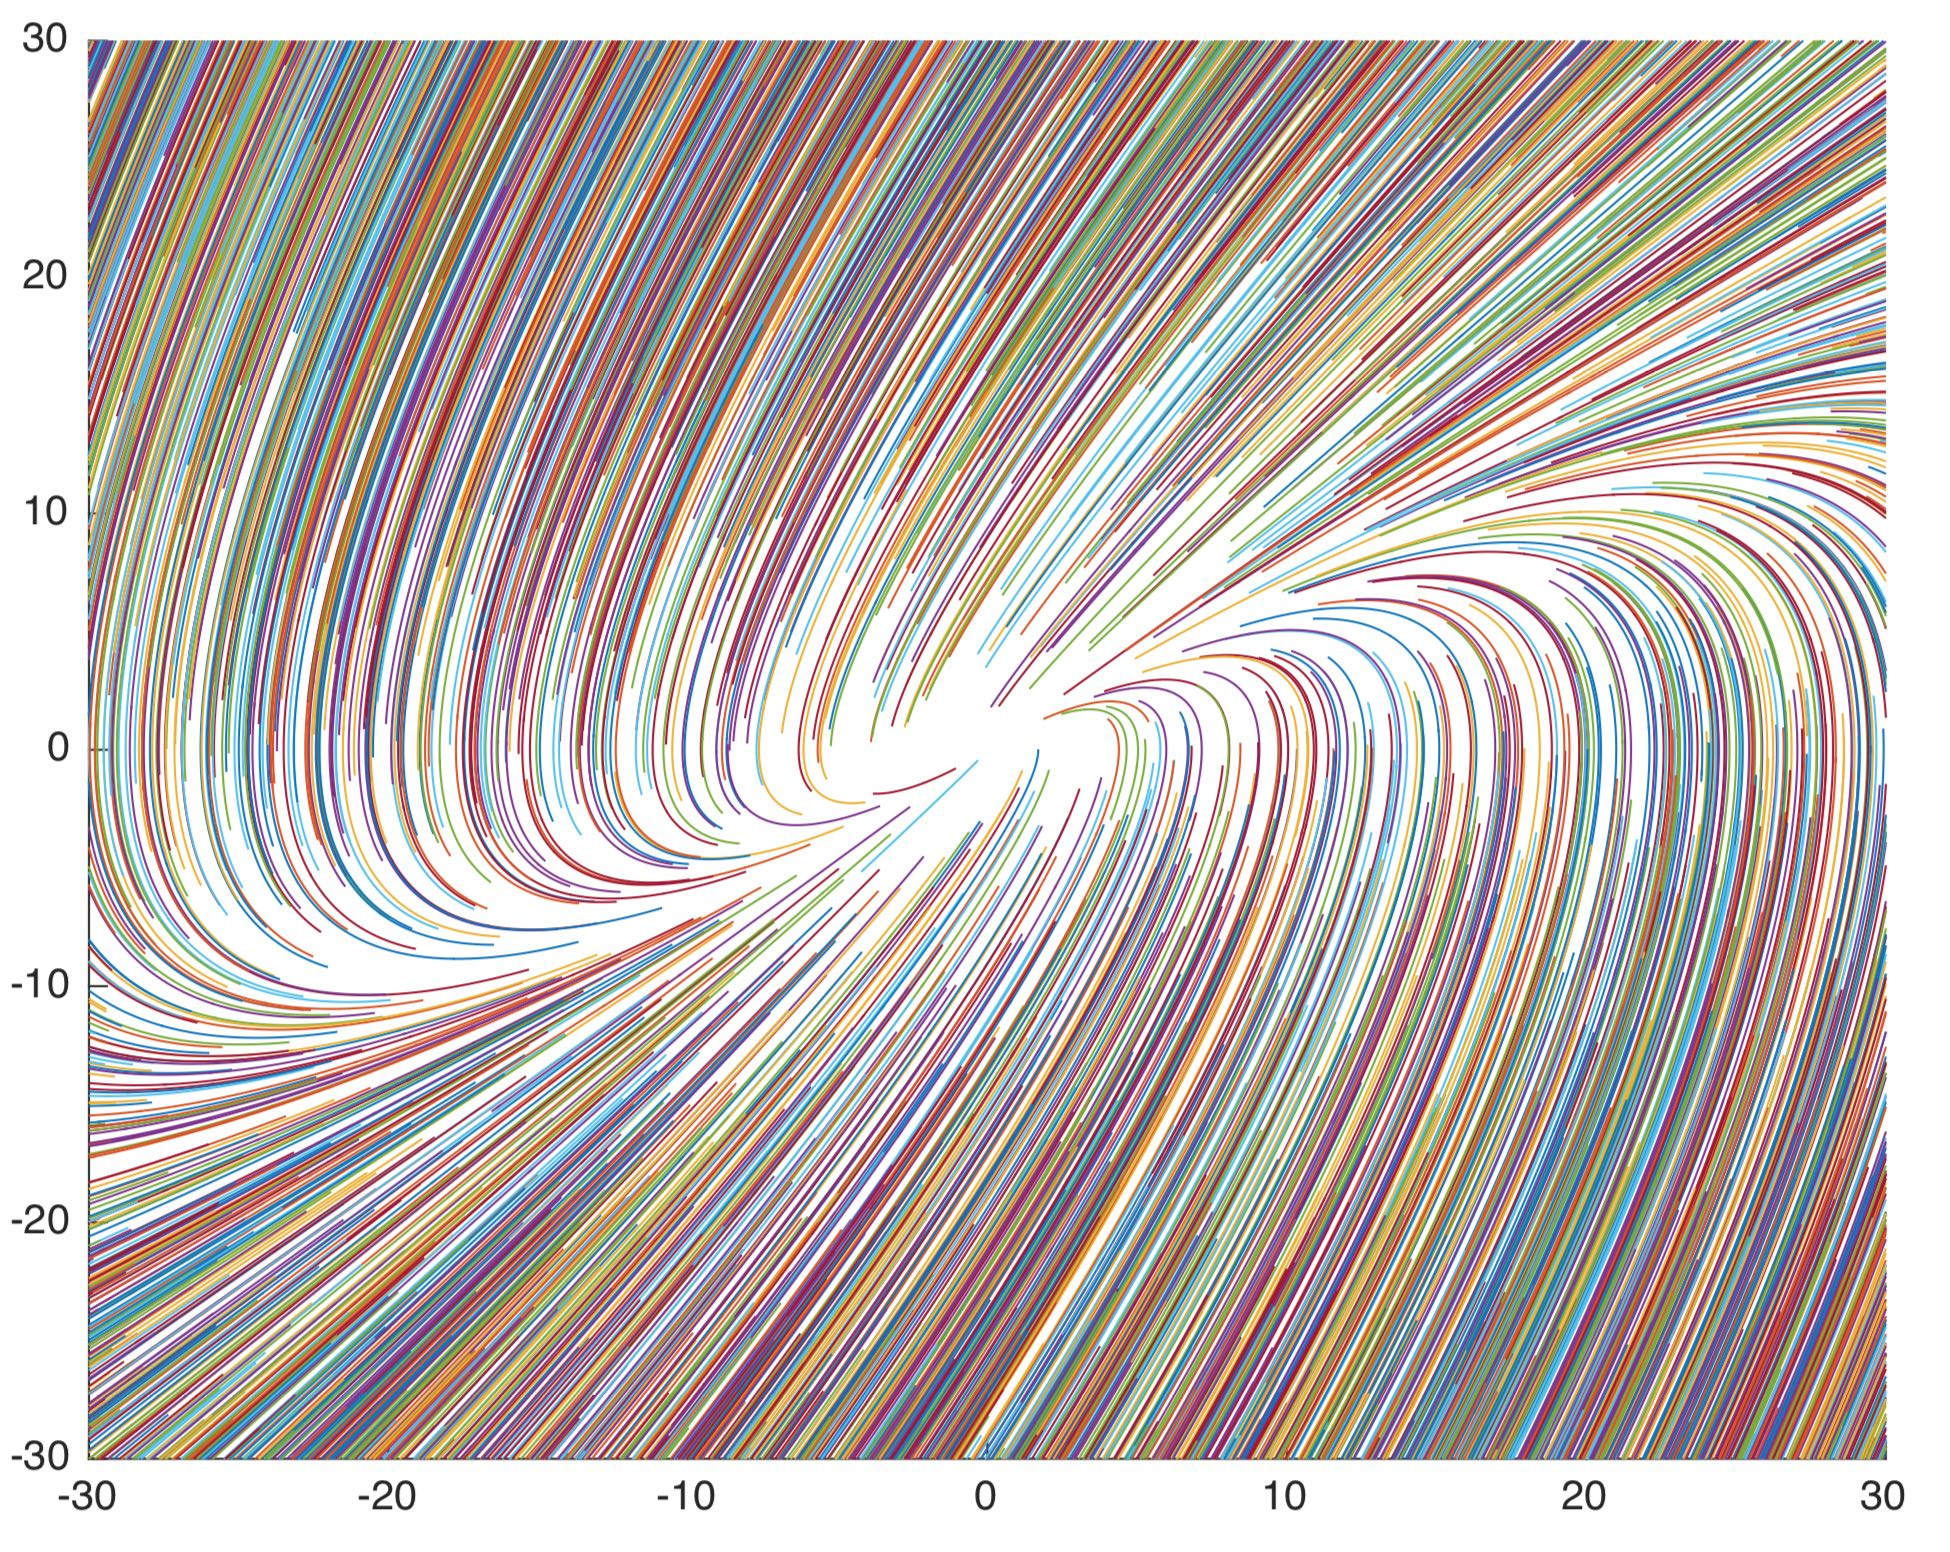
\includegraphics[scale=.1]{eks_6.jpg}
	\captionsetup{labelformat=empty}
	\caption{Eksempel \ref{eks_6}}
	\end{center}
\end{figure}


\kapittelslutt

